\newpage
\clearpage
\section{Results and Outlook}
    This is the $p_T$ spectrum of the yield for $\omega$ and $\phi$. Since the cross section has not been calculated for the vertical axis yet, a comparison with other experimental results cannot be made. However, a distribution with an exponential dependence on $p_T$ can be observed.
    \begin{figure}[htbp]
        \centering
        % Left side figure
        \begin{minipage}{0.45\textwidth} % Specify width using minipage
            \centering
            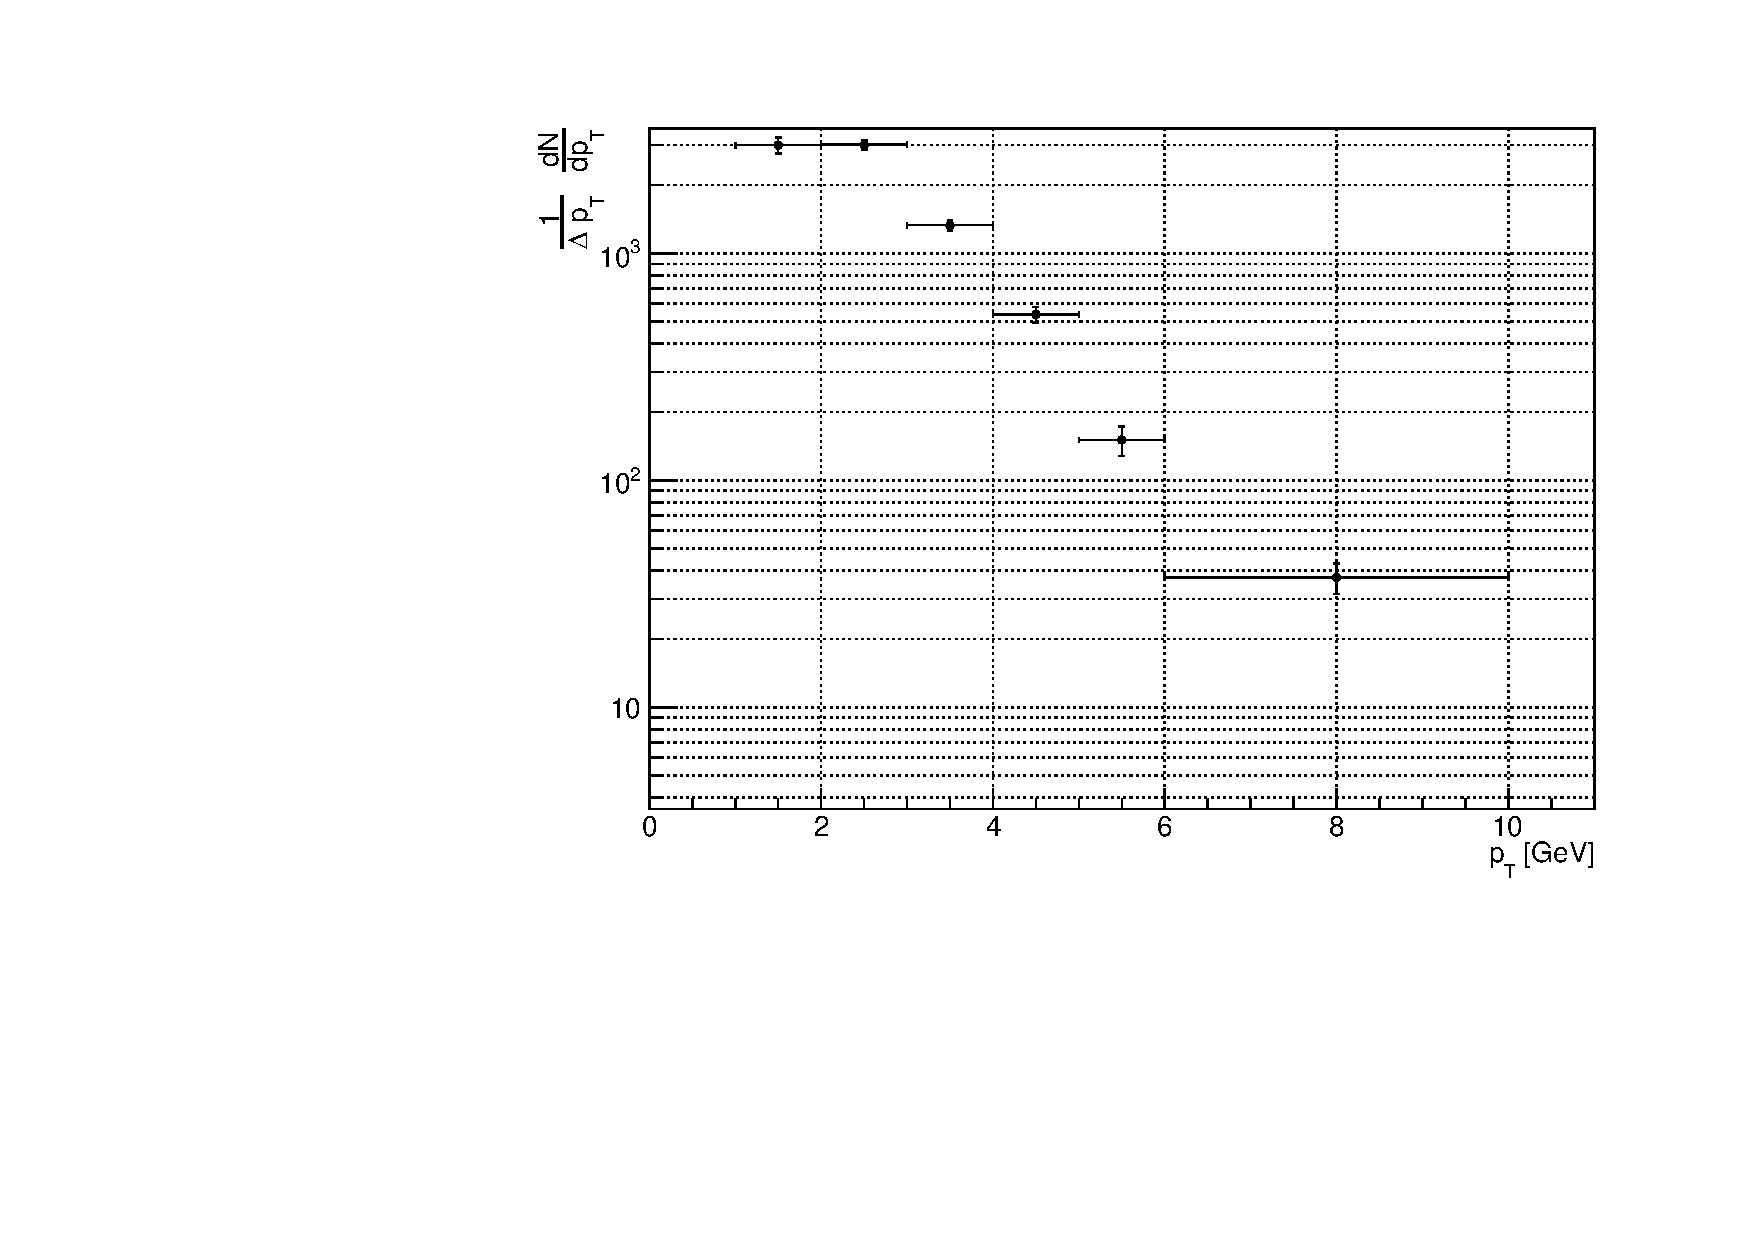
\includegraphics[width=\textwidth]{fig/4_omega_yield.pdf} % Left side image
            \caption{$\omega$ yield}
            \label{fig:omega_yield}
        \end{minipage}
        % Right side figure
        \hfill
        \begin{minipage}{0.45\textwidth}
            \centering
            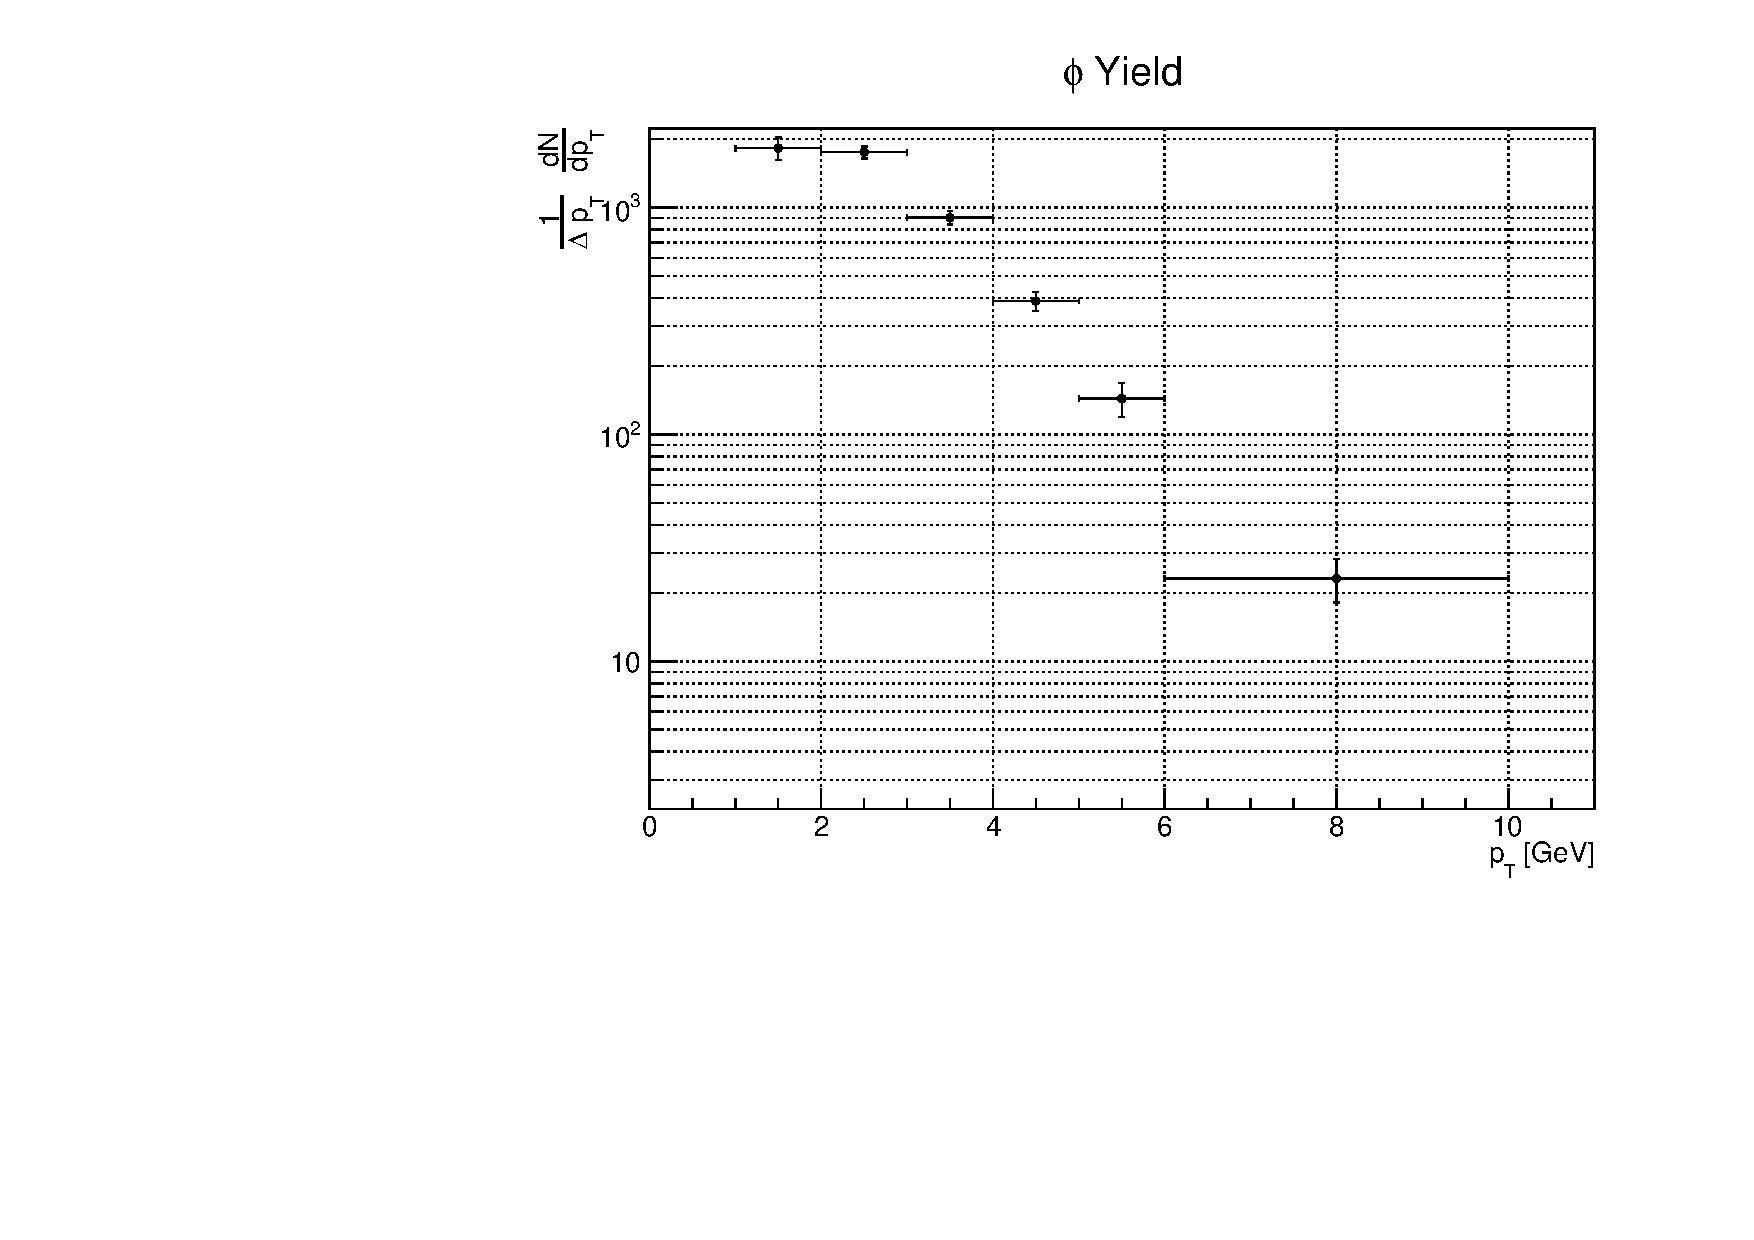
\includegraphics[width=\textwidth]{fig/4_phi_yield.pdf} % Right side image
            \caption{$\phi$ yield}
            \label{fig:phi_yield}
        \end{minipage}
    \end{figure}
    Since no corrections have been applied, a physical discussion cannot. however, a decreasing trend with increasing transverse momentum can be observed.  
    In this analysis, the results were obtained using the most standard cuts applied to muon tracks reconstructed with the tracking quality of the 2024. Additionally, the peak extraction for \( \omega \rightarrow \mu\mu \) and \( \phi \rightarrow \mu\mu \) was performed using a simple Gaussian function. Therefore, the yield calculation for \( \omega \) and \( \phi \) provides only a rough estimate. Further improvements in precision can be expected through enhancements in the single muon tracking quality and the use of fit functions that better represent the actual mass distribution.  
    Moreover, it is important to note that the \( \rho \rightarrow \mu\mu \) distribution is located near the \( \omega \rightarrow \mu\mu \) mass distribution. The \( \rho \) meson has a mean mass of \( m = 775.26 \) MeV and a full width of \( \Gamma = 149.1 \) MeV, meaning that it forms a broader distribution near the \( \omega \) peak. In this analysis, due to the broad distribution of \( \rho \) and the use of a simple fit function, the extraction of the \( \omega \) peak may have included contributions from \( \rho \) as well. 
    Looking ahead, improvements in the resolution of single muon kinematic variables are expected to enhance the mass resolution, leading to a sharper \( \omega \) peak. This would allow for better separation of the \( \rho \) and \( \omega \) peaks.

    Discuss single muon track reconstruction, \ref{matching improvements}, and future prospects as well. In the current muon track reconstruction algorithm, the pseudorapidity (\(\eta\)) and azimuthal angle (\(\phi\)) of the muon are determined using the MFT standalone track to improve their precision. However, the DCA is calculated using parameters obtained from the global fit of the MFT-MCH-MID track. Since using tracks closer to the collision point allows for more precise measurements unaffected by the absorber, it is expected that the accuracy of the DCA measurement can be improved by using the parameters of the MFT track that constitutes the MFT-MCH-MID track.Furthermore, improvements in MFT-MCH matching are also needed. As seen in \ref{purity_of_pt}, the matching purity significantly decreases at low transverse momentum (\( p_T \)). This degradation occurs because low-\( p_T \) muons undergo multiple scattering and energy loss in the absorber, making MFT-MCH matching more challenging. However, this study demonstrated that applying a \( \Delta \eta \) cut improves matching purity in the low-\( p_T \) region. This result suggests that continued analysis can further enhance matching purity.

    The ultimate goal is to measure the changes in the mass distribution of light vector mesons in lead-lead collision events. This study has revealed several remaining challenges, including issues with matching purity at low transverse momentum and the development of the track reconstruction algorithm. Additionally, improving the quality of muon tracks in high-multiplicity events in heavy-ion collisions is another challenge. As a first step, efforts will be focused on improving matching purity and developing the track reconstruction algorithm in proton-proton collisions, where the event multiplicity is relatively low. Subsequently, similar improvements will be pursued in heavy-ion collisions. Ultimately, the aim is to clarify the changes in the mass distribution of light vector mesons due to QGP formation and observe the restoration of chiral symmetry.
\section{Summary}
    In this study, we analyzed forward muon pairs in ALICE from $\sqrt{s} = 13.6$ TeV $pp$ collisions. The peaks corresponding to $\omega \rightarrow \mu\mu$ and $\phi \rightarrow \mu\mu$ in the dimuon mass distribution were extracted by fitting them with Gaussian functions, while other components were fitted with an exponential function. These analyses were performed for each transverse momentum range, and the transverse momentum spectra of $\omega$ and $\phi$ yields were presented. Additionally, an analysis was conducted to improve the matching purity between the MFT, introduced in Run 3, and the downstream detectors. By applying a cut on the difference in $\eta$ between the MFT Track and the MCH Track that constitute the Global Track, we demonstrated the ability to remove Fake Match tracks. Furthermore, the optimal MFT-MCH matching $\chi^2$ cut was determined using the signal yields of $\omega$ and $\phi$. As a future prospect, further improvements in the quality of Single Muon Tracks will be pursued. Ultimately, this study aims to clarify the changes in the mass distribution of light vector mesons caused by the formation of the QGP in lead-lead nuclear collisions.